\documentclass[a4paper,11pt]{article}

% Identificação
\newcommand{\pbtitulo}{Dash - Plotly}
\newcommand{\pbversao}{1.0}

\usepackage{../sty/tutorial}

%----------------------------------------------------------------------
% Início do Documento
%----------------------------------------------------------------------
\begin{document}
	
	\maketitle % mostrar o título
	\thispagestyle{fancy} % habilitar o cabeçalho/rodapé das páginas
	
%--------------------------------------------------------------------------
% RESUMO DO ARTIGO
%--------------------------------------------------------------------------
\begin{abstract}
	% O primeiro caractere deve vir com \initial{}
	\initial{D}ash \cite{dashoficial}, pode ser facilmente comparado ao \textit{Shiny} do R. Ambos possuem o mesmo objetivo a geração de páginas interativas (como Dashboards) para visualização dos dados. Criado totalmente com Python e se fossemos resumi-lo em três simples palavras diríamos: Interatividade, Incorporabilidade e Estética. Em poucas linhas de código é possível criar uma visão dos dados de modo que o usuário possa pensar que passamos o ano inteiro em sua montagem. E realmente isso fazia falta no Python.
\end{abstract}

%--------------------------------------------------------------------------
% CONTEÚDO DO ARTIGO
%--------------------------------------------------------------------------
\section{Parte inicial}
Gráficos em Python não são nenhuma novidade, desde 2003 temos a MatPlotLib, mas de uns anos, mais especificamente em 2012, surgiram a \textit{Bokeh} e \textit{Seaborn} o que começou a ficar interessante. Porém criar um dashboard completo ainda exigia muitas linhas de codificação e conhecimento. 

Antes de começarmos a falar realmente do Dash, vamos entender a empresa por trás do produto. \textit{Plotly}, sede em Montreal (Canadá), desenvolve ferramentas de análise e visualização de dados. Não pensemos que é restrito a Python, seu cartel de linguagens abrange R, MATLAB, Perl, Julia, Arduino e REST (garanto que até o momento imaginava que se tratava de uma simples sub biblioteca dentro do MatPlotLib).
\begin{figure}[H]
	\centering
	
\includegraphics[width=0.3\textwidth]{imagem/logo}
	\caption{Logo do Dash}
\end{figure}

\textbf{Dash}, é um produto \textit{Open Source} no qual existem versões tanto comerciais (\textit{Open Source} comercial? Sim, se ganha dinheiro com a prestação de assistência e suporte) quanto da comunidade. Assim sendo, Dash é uma biblioteca \textit{Open Source}, liberada sob a licença MIT (veja mais em \url{https://opensource.org/licenses/MIT}). Quando o Dash é executado por trás existe um servidor \textit{Flask} e na verdade podemos dizer que trata-se de uma extensão desse servidor.

Só para esclarecermos quem não entende muito de tecnologias, sem o Dash temos que criar algum tipo de estrutura com o \textit{PyQt} ou \textit{Tkinter}, ativar um Servidor Web como \textit{Flask} ou \textit{Django}, e depois combiná-lo com estruturas \textit{JavaScripts} interativas para incorporar interatividade, provavelmente \textit{jQuery}. Isso levaria bastante tempo, esforço e principalmente código. O Dash já encapsula tudo isso. De fato, Dash estende o \textit{Flask} e toda vez que criamos algo, na verdade, estamos em um aplicativo \textit{Flask} mas sem a menor necessidade de sabermos nada a respeito dele.

Antes de começarmos será necessário 2 conhecimentos que não abordaremos nessa apostila, obviamente Python e HTML a nível básico (talvez até um pouco de CSS). Veremos que não existe nada em Dash que possa assustar sendo que o programa criado possui uma estrutura limpa e coesa. Como editor utilizaremos o \textit{PyCharm} \cite{pycharmoficial} (versão da Comunidade) da \textbf{JetBrains}.

\section{Instalação do Ambiente}
Vamos partir que o Python (versão 3.x) já está instalado e configurado assim como PyCharm. Para o Dash uma única linha de código é necessária: \\
\codigo{\$ pip install dash}

E estamos prontos para trabalhar. Vamos começar criando um novo projeto:
\begin{figure}[H]
	\centering
	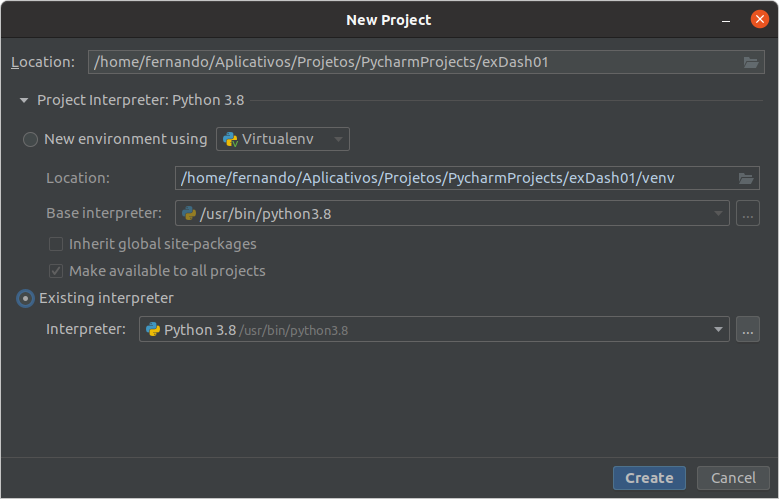
\includegraphics[width=0.6\textwidth]{imagem/novoProjeto}
	\caption{Novo Projeto no PyCharm}
\end{figure}

A parte mais importante quando criamos um novo projeto é garantir que o interpretador correto esteja marcado e apontado para a versão do Python que estamos trabalhando (normalmente vem marcado a opção para um ambiente virtual).

Criamos um programa em Python para verificarmos se tudo funciona corretamente (\textit{exemplo01.py}):
\begin{lstlisting}[]
import dash
import dash_core_components as dcc
import dash_html_components as html

print('Dash:', dash.__version__)
print('Core:', dcc.__version__)
print('HTML:', html.__version__)
\end{lstlisting}

Clicar com o botão direito do mouse e selecionar a opção: \opcbotao{Run 'exemplo01.py'}. E obtemos a seguinte resposta na saída da console: \\
\codigo{Dash: 1.13.3 \\
	Core: 1.10.1 \\
	HTML: 1.0.3}

Dash possui 3 bibliotecas distintas: \textbf{dash} (que como já citamos é uma extensão do Servidor Web), \textbf{core} (seus elementos principais) e \textbf{html} (como o nome diz são as tags HTML que utilizaremos para estruturar nosso \textit{Dashboard}). E podemos seguir adiante.

\section{Biblioteca HTML}
A biblioteca \textit{dash\_html\_components} é a parte que interagimos com o HTML. Pensemos nisso como uma estrutura (em árvore) de uma página qualquer. Faça uma visita no site \url{https://dash.plotly.com/dash-html-components} e veja a documentação completa. Quando iniciamos em qualquer linguagem temos que criar um programa que mostre um "Hello World!" na tela (isso é de praxe) então para não ofendermos aos deuses da programação (livrai-nos dos Bugs. Amém!) vamos criá-lo, criamos um novo programa (\textit{exemplo02.py}):
\begin{lstlisting}[]
import dash
import dash_core_components as dcc
import dash_html_components as html

app = dash.Dash()

app.layout = html.Div([
  html.H1("Hello World!")
])

if __name__ == "__main__":
  app.run_server(debug=True)
\end{lstlisting}

Nosso servidor está representado pela variável \textit{app}, para esta na seção \textit{layout} montamos toda nossa estrutura, essa deve possuir uma raiz HTML (tag DIV), no caso deste exemplo, adicionamos uma tag H1 colocamos a palavra \aspas{Hello World!}. Ao executarmos esse programa na saída da console observamos a seguinte mensagem: \\
\codigo{* Running on http://127.0.0.1:8050/ (Press CTRL+C to quit)}

No navegador ao abrirmos o endereço indicado temos:
\begin{figure}[H]
	\centering
	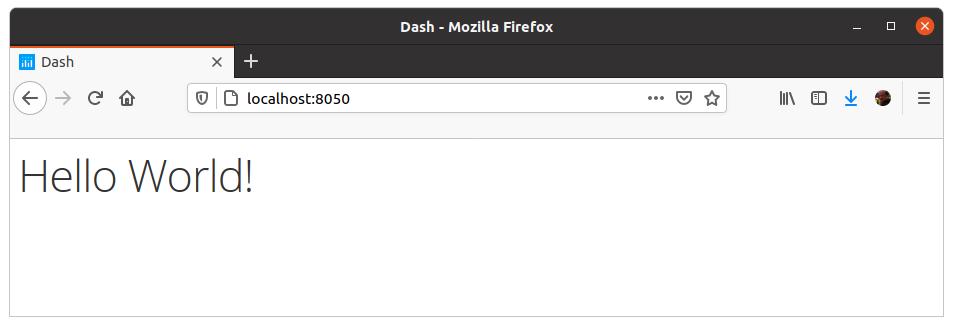
\includegraphics[width=0.6\textwidth]{imagem/hello}
	\caption{Hello World no Dash}
\end{figure}

Por padrão o servidor é 127.0.0.1 (localhost) e a porta 8050. Mas podemos modificar isso através da seguinte codificação: \\
\codigo{app.run\_server(port=8050, host=\aspas{127.0.0.1})}

Ao rodar o servidor com a opção \textit{debug=True} estamos dizendo para este: qualquer alteração que realizemos deve se atualizar automaticamente. Isso é conhecido como \textit{HotFix}. Por exemplo, mudemos a palavra \aspas{Hello World!} para qualquer outra que desejemos e veremos que a página é modificada (inclusive sem a necessidade de aplicarmos um \textit{refresh} no navegador).

Ao invés de repetirmos todo o programa ao longo dessa apostila, consideremos que a partir desse ponto tudo o que escrevemos segue a seguinte estrutura:
\begin{lstlisting}[]
...
[ NOVAS BIBLIOTECAS ]

app = dash.Dash()

[ COMANDOS AQUI ]

if __name__ == "__main__":
  ...
\end{lstlisting}

Lembremos também que para cada programa novo criado, devemos interromper a execução do anterior para evitarmos o conflito das portas.

\subsection{Adição de Gráficos}
Vamos adicionar as bibliotecas necessárias: \\
\codigo{import random \\
import pandas as pd}

Temos a \textit{random} somente para termos dados aleatórios e a \textit{Pandas} para montarmos nossos em um \textit{DataFrame} (não é necessário, mas tornamos nosso exemplo mais consistente). Para a montagem dos dados adicionar a seguinte codificação:
\begin{lstlisting}[]
ano = []
qtdMoto = []
qtdCarro = []
for i in range(2010, 2021):
  ano.append(i)
  qtdMoto.append(random.randint(0, 100))
  qtdCarro.append(random.randint(0, 100))
  
df = pd.DataFrame({
  "Ano": ano,
  "Carro": qtdCarro,
  "Moto": qtdMoto
})
\end{lstlisting}

Criamos três listas: ano (que conterá os anos entre 2010 a 2020), qtdMoto (quantidade de motos nesse período) e qtdCarro (quantidade de carros nesse período) e as colocamos em colunas montando o \textit{dataframe} final. Para mostrá-los de forma gráfica:

\begin{lstlisting}[]
app.title = 'Motos e Carros'
app.layout = html.Div([
  html.H1("Veículos Brasil"),
  html.Div([
    dcc.Graph(
      id='principal',
      figure={
  	    'data': [
	      {'x': df.Ano, 'y': df.Moto, 'type': 'line', 'name': 'Motos'},
	      {'x': df.Ano, 'y': df.Carro, 'type': 'bar', 'name': 'Carros'},
	    ],
	    'layout': {
	      'title': 'Comparativo entre Carros e Motos'
	    }
      }
    ),
  ]),  # DIV principal
])
\end{lstlisting}

O atributo \textit{title} se refere ao título do site. Adicionamos mais um componente (\textit{dcc}) que contém nosso gráfico. Criamos uma tag HTML DIV somente para termos uma divisão lógica no nosso HTML principal. O gráfico é criado a partir do componente (DCC) \textit{Graph} que obrigatoriamente este deve ter uma chave única (id), o parâmetro \textit{figure} é dividido em duas seções: data (que contém nossos dados e detalhes do gráfico) e layout (com as características da figura). E obtemos o seguinte resultado:
\begin{figure}[H]
	\centering
	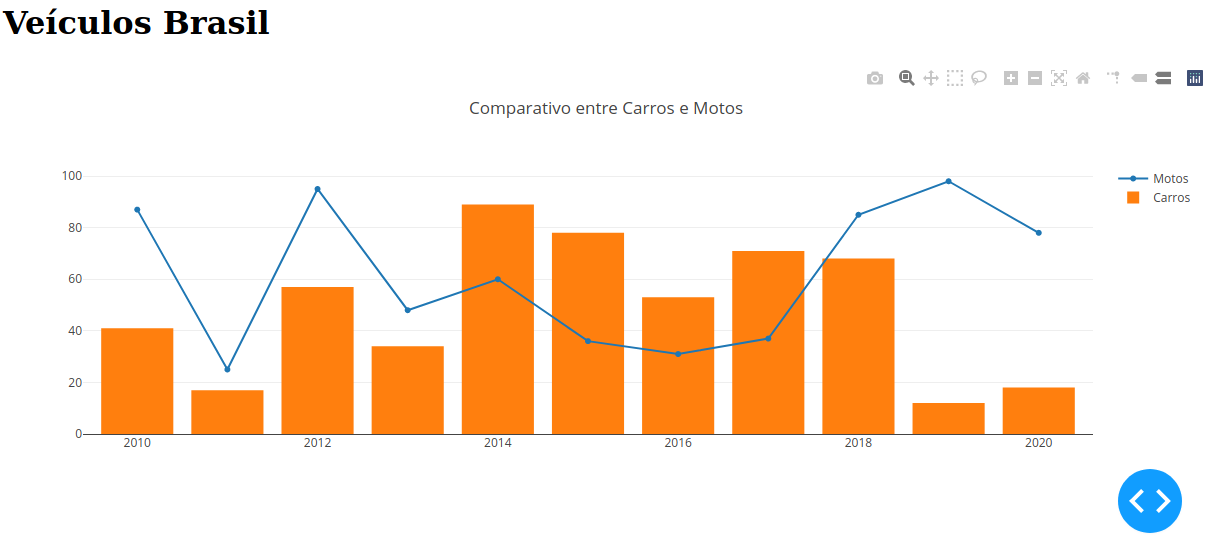
\includegraphics[width=0.8\textwidth]{imagem/grafico1}
	\caption{Gráfico no Dash}
\end{figure}

Ao posicionarmos o mouse sobre o gráfico vemos que aparece uma barra de opções superior no qual podemos realizar download da imagem, aplicar um Zoom, entre algumas outras opções. Se percorremos com o mouse veremos que as quantidades de cada um dos tipos é mostrada, na lateral superior a direita está a legenda e na parte inferior um botão azul (este aparece somente pois estamos em modo \textit{debug}) que indica o estado do nosso servidor. Toda essa interatividade é permitida pois na camada visual existe o \textit{React.js}. Além disso nosso site é completamente responsivo, se o reduzimos observamos que os elementos automaticamente se adaptam.

Obviamente por se tratar de dados aleatórios esta imagem pode ser modificada. Além disso percebemos que com poucas linhas de código já temos a condição de criar um DashBoard como quisermos. A galeria de gráficos que temos a nossa disposição possui uma boa variedade e pode ser acessa em \url{https://dash-gallery.plotly.host/Portal/}.

\subsection{Adição de CSS}
CSS (\textit{Cascading Style Sheet}) é utilizado em aplicações HTML para "estilizar" a página. Normalmente isso fica a cargo do Web Designer, mas o que é mais impressionante que podemos adicioná-los ao nosso gráfico sem criar absolutamente nada no código, para isso devemos criar uma subpasta no nosso projeto chamada /assets e nesta podemos adicionar imagens ou arquivos CSS que serão automaticamente lidos.

No PyCharm, menu lateral a esquerda clicar com o botão direito sobre o projeto e selecionar as opções \opcmenu{New } $\triangleright$ \opcmenu{Directory}. Informar o nome \opcbotao{assets } e pressionar \textbf{Enter}. No site \url{https://codepen.io/chriddyp/pen/bWLwgP.css} baixar o arquivo para este diretório. Parar o programa e executar novamente (este é um dos casos aonde o \textit{refresh} automático de página não funciona). E observamos que o estilo do título \aspas{Veículos Brasil} foi modificado para:
\begin{figure}[H]
	\centering
	
\includegraphics[width=0.2\textwidth]{imagem/tituloSite}
	\caption{Tipografia do Título}
\end{figure}

Mas não apenas isso, temos opções bem interessantes, como por exemplo o modo colunar. Vamos imaginar que desejamos mais dois gráficos abaixo desse e uma tabela com a amostragem dos dados. Primeiro abaixo dos \textit{imports} vamos criar a seguinte função que monta a tabela:
\begin{lstlisting}[]
def generate_table(dataframe, max_rows=11):
  return html.Table([
    html.Thead(
    html.Tr([html.Th(col) for col in dataframe.columns])
  ),
  html.Tbody([
    html.Tr([
      html.Td(dataframe.iloc[i][col]) for col in dataframe.columns
    ]) for i in range(min(len(dataframe), max_rows))
  ])
])
\end{lstlisting}

Fizemos algo mais genérico pois reaproveitamos esse método para outros \textit{dashboards}. Os parâmetros passados são o \textit{dataframe} e número máximo de linhas a mostrar. Próximo passo é a montagem:
\begin{lstlisting}[]
    ...
  ]),  # DIV principal
  html.Div([
    html.Div([
      generate_table(df),
    ], className='two columns'),
    html.Div([
      dcc.Graph(
        id='boxMoto',
        figure={
          'data': [{
             'name': 'Dispersão',
             'y': df.Moto,
             'type': 'box',
          }],
          'layout': {
            'title': 'Motos'
          }
        }
      ),
    ], className='five columns'),
    html.Div([
      dcc.Graph(
        id='boxCarro',
        figure={
          'data': [{
            'name': 'Dispersão',
            'y': df.Carro,
            'type': 'box',
          }],
          'layout': {
            'title': 'Carros'
          }
        }
      ),
    ], className='five columns'),
  ])
])
\end{lstlisting}

Ao término do DIV para o elemento "principal" criamos mais uma DIV que conterá nossa estrutura. O primeiro DIV chama o método criado para obtermos nossa tabela, na opção \textit{className} indicamos quantas colunas (num total imaginário de doze) ocupa (no caso duas). O próximo DIV conterá um gráfico tipo \textit{BoxPlot} para mostrar a dispersão dos dados de Motos e o último de carros, sendo que cada um ocupa cinco colunas. E obtemos o seguinte resultado abaixo do nosso gráfico principal:
\begin{figure}[H]
	\centering
	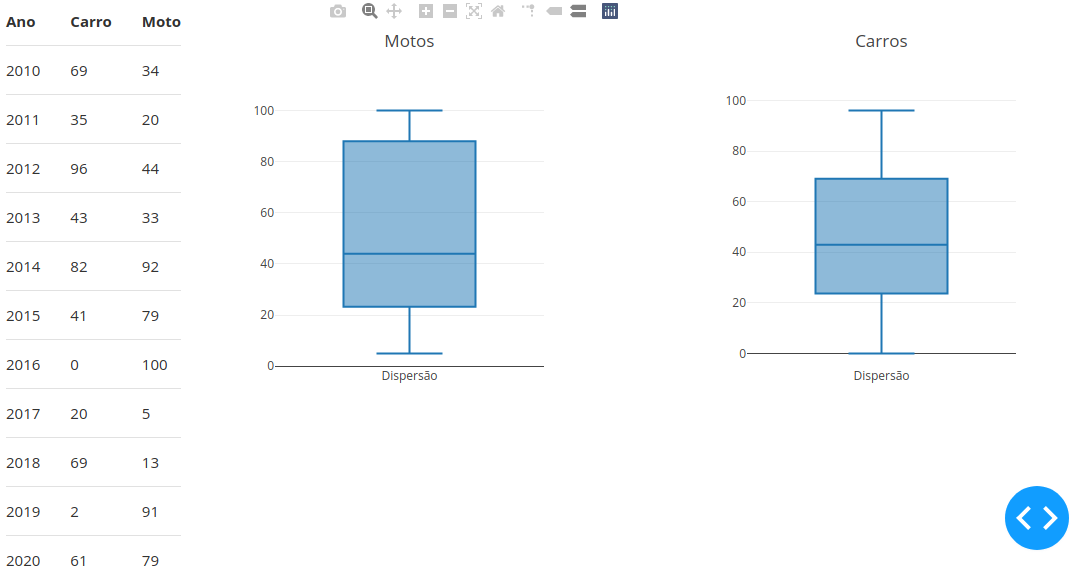
\includegraphics[width=0.7\textwidth]{imagem/baixo}
	\caption{Detalhes da parte inferior}
\end{figure}

Posicionamos o mouse sobre qualquer um dos \textit{boxplots} e obtemos todas as medidas que formam esse.

\section{Biblioteca de Componentes}
A biblioteca \textit{dash\_core\_components} permite além dos gráficos que já vimos, elementos como \textit{dropdowns}, caixas de texto entre muitos outros. Faça uma visita no site \url{https://dash.plotly.com/dash-core-components} e veja a lista completa.

Vamos começar com a importação da biblioteca necessária para "colar" o componente: \\
\codigo{from dash.dependencies import Input, Output}

Vamos adicionar um RangeSlider ao gráfico principal que será responsável por controlar o Intervalo Anual mostrado neste:
\begin{lstlisting}[]
  ...
  html.H1('Veículos Brasil'),
  html.Div([
    html.Label('Intervalo Anual'),
    dcc.RangeSlider(
      id='rangeAnual',
      min=min(df.Ano),
      max=max(df.Ano),
      marks={i: 'Ano {}'.format(i) if i == min(df.Ano) else str(i) for i in range(min(df.Ano), max(df.Ano))},
      value=[min(df.Ano), max(df.Ano)],
    ),
    html.Div([
      dcc.Graph(id='principal'),
    ]),
  ]),  # DIV principal
  ...
\end{lstlisting}

Não nos preocupemos agora do gráfico ter perdido todos seus elementos, pois como será dinâmico esses foram transferidos. Lembremos da importância de cada elemento ter um ID, pois são esses que realizam a interação entre eles. Abaixo de toda essa estrutura do "app.layout" criamos um método com a anotação \textit{app.callback}:
\begin{lstlisting}[]
@app.callback(Output('principal', 'figure'), [
  Input('rangeAnual', 'value'),
])
def modifica_principal(rangeAnual):
  return {
    'data': [
      {'x': df.Ano, 'y': df.Moto, 'type': 'line', 'name': 'Motos'},
      {'x': df.Ano, 'y': df.Carro, 'type': 'bar', 'name': 'Carros'},
    ],
    'layout': {
      'title': 'Comparativo entre Carros e Motos',
      'xaxis': {
        'range': [rangeAnual[0], rangeAnual[1]]
      },
    }
  }
\end{lstlisting}

Temos neste dois elementos: Entradas (\textit{Input}) e Saída (\textit{Output}). Podemos ter várias chamadas (\textit{callback}) para os diversos gráficos do \textit{dashboard} mas cada uma deve se referir a um único elemento de saída. É realizado dessa forma pois essa chamada automaticamente (na mudança dos valores dos elementos de entrada) realiza a chamada do método descrito abaixo deste.

Neste método colocamos todos os componentes para construirmos a figura para o gráfico (definido pelo \textit{Output}) e acertamos seus  parâmetros conforme a informação enviada (no caso o intervalo de valores). Obtemos agora a seguinte visualização:
\begin{figure}[H]
	\centering
	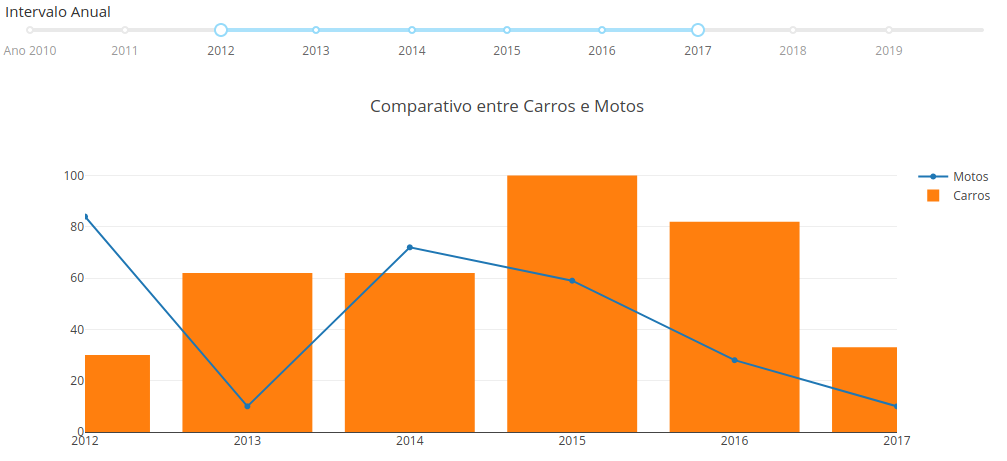
\includegraphics[width=0.7\textwidth]{imagem/parametro}
	\caption{Entrada de Valores Anuais}
\end{figure}

Para este componente \textit{SliderRange} podemos arrastar tanto o início quanto final que o gráfico se adaptará as mudanças. Como exercício prático tente modificar os outros componentes para que se comportem também de acordo, lembrando que é um \textit{callback} para cada componente gráfico.

\subsection{Novas Interações}
Dessa vez vamos criar um exemplo completo com um gráfico totalmente interativo:
\begin{lstlisting}[]
import dash
import dash_core_components as dcc
import dash_html_components as html
from dash.dependencies import Input, Output
import random

# Geração dos Dados
ano = []
dados = []
for i in range(2010, 2021):
  ano.append(i)
  dados.append(random.randint(10, 500))

# Montagem do Layout
app = dash.Dash()
app.layout = html.Div([
  html.Div([
    html.Div([
      dcc.Dropdown(
        id='cor',
        options=[i for i in [
          {'label': 'Azul Metal', 'value': '#4682B4'},
          {'label': 'Salmão', 'value': '#FA8072'},
          {'label': 'Verde Verão', 'value': '#00FF7F'},
          {'label': 'Rosa', 'value': '#FF14B3'},
          {'label': 'Oliva', 'value': '#808000'},
          {'label': 'Siena', 'value': '#A05220'}
        ]],
        value='#2ECC40'
      )
    ], className="six columns"),
    html.Div([
      dcc.Slider(
        id='tamanho',
        min=5,
        max=50,
        marks={i: 'Tamanho {}'.format(i) if i == 5 else str(i) for i in range(5, 50, 5)},
        value=20
      )
    ], className="six columns"),
  ], className="row"),
  html.Div([
    dcc.Graph(id='central'),
  ]),
])

# Modificações no Gráfico
@app.callback(Output('central', 'figure'), [
  Input('cor', 'value'),
  Input('tamanho', 'value'),
])
def alterar_central(cor, tamanho):
  return {
    'data': [{
      'x': ano,
      'y': dados,
      'type': 'scatter',
      'mode': 'markers',
      'marker': {
        'color': cor,
        'size': tamanho
      }
    }],
    'layout': {
      'xaxis': {'range': [min(ano)-1, max(ano)+1]},
      'yaxis': {'range': [10, 500]},
      'transition': {
        'duration': 500,
        'easing': 'cubic-in-out'
      }
    }
  }

if __name__ == '__main__':
  app.run_server(debug=True)
\end{lstlisting}

Importamos as bibliotecas necessárias e criamos os dados (um conjunto de anos e valores aleatórios que variam de 10 a 500). A montagem do nosso layout é composto por duas partes: na primeira superior temos um componente de \textit{Dropdown} (caixa de escolha) com as características de cor e ao seu lado um \textit{Slider} de modo que possamos aumentar ou diminuir o tamanho dos pontos mostrados no gráfico (mínimo de 10 e máximo 50); na segunda parte central temos o gráfico.

Com as mudanças dos elementos \textit{Dropdown} ou \textit{Slider} é disparado o método \textbf{alterar\_central()} que realiza a mudança das características do gráfico (observar o parâmetro \textit{marker}). O parâmetro \textit{transition} realiza uma mudança suave (ao invés de instantânea). Obtemos como resultado:
\begin{figure}[H]
	\centering
	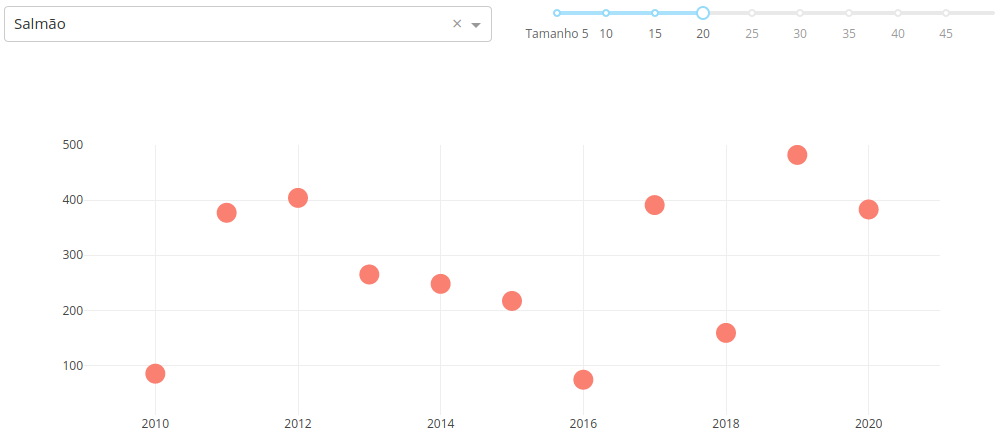
\includegraphics[width=0.5\textwidth]{imagem/interacao}
	\caption{Modificação das Características do Gráfico}
\end{figure}

E agora estamos prontos para mostrar nossos dados através de um Servidor Web dinâmico.

\section{Conclusão}
Aplicativos Dash são Servidores Web que estende o \textit{Flask}. Flask é amplamente adotado pela comunidade Python e implantado em ambientes de produção. Para os desenvolvedores avançados, Dash ainda permite ser estendido por meio de plug-ins do Flask. A camada visual processa componentes através do \textit{React.js}, a biblioteca de interface \textit{Javascript} criada e mantida pelo \textit{Facebook}. 

O layout descreve como é a visualização. Montado como uma árvore hierárquica de componentes. A biblioteca \textit{dash\_html\_components} fornece classes para todas as tags HTML e seus atributos como estilo e id. A biblioteca \textit{dash\_core\_components} gera componentes de nível superior, como controles e gráficos. Seu domínio facilita a construção de qualquer \textit{dashboard} que necessitemos.

Sou um entusiasta do mundo \textbf{Open Source} e novas tecnologias. Qual a diferença entre Livre e Open Source? \underline{Livre} significa que esta apostila é gratuita e pode ser compartilhada a vontade. \underline{Open Source} além de livre todos os arquivos que permitem a geração desta (chamados de arquivos fontes) devem ser disponibilizados para que qualquer pessoa possa modificar ao seu prazer, gerar novas, complementar ou fazer o que quiser. Os fontes da apostila (que foi produzida com o LaTex) está disponibilizado no GitHub \cite{github}. Veja ainda outros artigos que publico sobre tecnologia através do meu Blog Oficial \cite{fernandoanselmo}.

%--------------------------------------------------------------------------
% REFERÊNCIAS
%--------------------------------------------------------------------------
\begin{thebibliography}{4}
	\bibitem{dashoficial} 
	Página do Dash \\
	\url{https://plotly.com/dash/}

	\bibitem{pycharmoficial} 
	Página do PyCharm \\
	\url{https://www.jetbrains.com/pt-br/pycharm/download/#section=linux}
	
		\bibitem{fernandoanselmo} 
	Fernando Anselmo - Blog Oficial de Tecnologia \\
	\url{http://www.fernandoanselmo.blogspot.com.br/}
	
	\bibitem{publicacao} 
	Encontre essa e outras publicações em \\
	\url{https://cetrex.academia.edu/FernandoAnselmo}
	
	\bibitem{github} 
	Repositório para os fontes da apostila \\
	\url{https://github.com/fernandoans/publicacoes}
\end{thebibliography}

\end{document}